\capitulo{3}{Conceptos teóricos}
En esta sección se presentan los fundamentos teóricos necesarios para comprender el desarrollo y la implementación del presente Trabajo de Fin de Grado. Se abordan las principales definiciones, teorías y modelos que sustentan la investigación, así como las tecnologías y herramientas empleadas. 
\section{Realidad virtual}
Se entiende por realidad virtual (VR) la tecnología que permite crear entornos digitales tridimensionales, interactivos y en tiempo real, de forma que el usuario perciba la sensación de “estar presente” en dicho entorno. Este grado de inmersión y “telepresencia” se consigue mediante la combinación de hardware (cascos HMD, sistemas de tracking, interfaces hápticas) y software (motores gráficos, algoritmos de simulación) que actualizan la escena virtual en función de los movimientos y acciones del usuario~\cite{steuer92,sherman2002}.

Dentro del estudio de la VR suelen distinguirse tres características fundamentales:

\textbf{Inmersión:} grado en que el sistema aísla y sustituye estímulos sensoriales reales por estímulos generados artificialmente, creando la impresión directa de “estar dentro” del entorno virtual~\cite{milgram94}.

\textbf{Presencia:} sensación subjetiva de “estar realmente” en el escenario virtual, más allá de la mera percepción sensorial~\cite{sherman2002,slater94}.

\textbf{Interactividad:} capacidad del sistema para registrar las acciones del usuario y modificar el entorno virtual de forma coherente y en tiempo real~\cite{steuer92,milgram94}.

Estas características hacen de la VR una herramienta poderosa en ámbitos tan diversos como la simulación de entrenamiento, la rehabilitación médica, la visualización arquitectónica o la investigación científica.

\subsection{Componentes de un sistema de VR}

Un sistema de VR típico se compone de los siguientes elementos~\cite{sherman2002,burdea2003}:
\begin{itemize}
  \item \textbf{Dispositivo de visualización (Head-Mounted Display, HMD):} muestra las imágenes estereoscópicas e incorpora sensores de orientación (giroscopios, acelerómetros).
  \item \textbf{Sistema de seguimiento (tracking):} rastrea la posición y orientación de la cabeza, manos u otros objetos mediante cámaras, emisores infrarrojos o sistemas magnéticos.
  \item \textbf{Dispositivos de interacción:} mandos, guantes hápticos o superficies táctiles que permiten manipular objetos virtuales.
  \item \textbf{Motor gráfico y software de simulación:} genera las escenas 3D, gestiona física, colisiones y comportamientos de los elementos del entorno.
\end{itemize}

\subsection{Taxonomía: Continuo de la virtualidad}

Milgram y Kishino propusieron el concepto de continuo de la virtualidad, que va desde la realidad completamente física hasta la realidad completamente virtual, englobando la realidad aumentada (AR) y la realidad mixta asistida~\cite{milgram94}:
\begin{itemize}
  \item \textbf{Realidad Aumentada (AR):} superposición de información virtual sobre el entorno real.
  \item \textbf{Realidad Mixta (MR):} fusión de elementos reales y virtuales que interactúan entre sí.
  \item \textbf{Realidad Virtual (VR):} reemplazo total del entorno real por uno virtual.
\end{itemize}

\subsection{Modalidades de uso y aplicaciones}

Según el grado de inmersión y el tipo de interacción, los sistemas de VR pueden clasificarse en:
\begin{itemize}
  \item \textbf{VR de escritorio:} utiliza pantallas convencionales y controladores estándar; menor inmersión, pero accesible.
  \item \textbf{VR inmersiva:} emplea HMDs y sistemas de tracking avanzado; alta inmersión y presencia~\cite{burdea2003}.
  \item \textbf{CAVEs:} espacios cerrados con pantallas proyectadas en paredes y suelo; múltiples usuarios simultáneos.
\end{itemize}

Las aplicaciones más difundidas incluyen simuladores de vuelo y conducción, terapias de exposición en salud mental, entrenamiento quirúrgico y entornos de aprendizaje inmersivo.

\section{Diseño de videojuegos para rehabilitación}

El uso de videojuegos para la rehabilitación física se enmarca dentro del concepto de \textit{serious games}, definido como aquellos juegos cuyo principal objetivo va más allá del entretenimiento, buscando también la educación, la formación o la mejora de la salud~\cite{david2016serious}.

\subsection{Principios de diseño}

El desarrollo de videojuegos para rehabilitación debe considerar aspectos tanto lúdicos como terapéuticos~\cite{greene2016rehab}. Entre los principales principios de diseño se encuentran:

\begin{itemize}
    \item \textbf{Interactividad:} permite al usuario manipular y explorar el entorno, facilitando el aprendizaje y la mejora de habilidades motoras.
    \item \textbf{\textit{Feedback} inmediato:} el sistema debe ofrecer respuestas instantáneas a las acciones del usuario, reforzando el progreso~\cite{cameirao2010impact}.
    \item \textbf{Dificultad progresiva:} las tareas deben adaptarse al nivel de capacidad del paciente, aumentando la complejidad de forma gradual para evitar la frustración~\cite{zimmerli2012virtual}.
    \item \textbf{Repetición y refuerzo positivo:} elementos clave en la rehabilitación física para promover la neuroplasticidad~\cite{holden2005virtual}.
\end{itemize}

\subsection{Gamificación y motivación}

La gamificación introduce mecánicas de juego (puntos, logros, niveles) que aumentan la motivación y el compromiso del usuario~\cite{sardi2017gamification}. En el caso del presente proyecto, la superación de puzles y la obtención de logros sirven como incentivo para continuar con las sesiones terapéuticas.

\subsection{Accesibilidad y consideraciones éticas}

Los videojuegos de rehabilitación deben garantizar la accesibilidad a personas con diferentes grados de discapacidad. Además, se debe asegurar que el uso de la tecnología no sustituya la supervisión profesional, sino que actúe como complemento ~\cite{rodriguez2020reha}.

\section{Teoría del aprendizaje motor}

La teoría del aprendizaje motor se basa en el modelo trifásico de Fitts y Posner~\cite{fitts1967}, que describe la adquisición de habilidades motoras en tres etapas:

\begin{enumerate}
  \item \textbf{Fase cognitiva:} el aprendiz construye una representación mental de la tarea, explorando secuencias de movimiento y cometiendo errores frecuentes. La ejecución es lenta y requiere alta atención consciente~\cite{schmidt2019}.
  \item \textbf{Fase asociativa:} se establecen mapeos más precisos entre estímulos y respuestas motoras. La variabilidad de la ejecución disminuye y se corrigen errores de forma más autónoma, consolidándose patrones de movimiento~\cite{schmidt2019}.
  \item \textbf{Fase autónoma:} la habilidad está completamente automatizada; la ejecución es rápida, fluida y apenas requiere atención consciente, liberando recursos cognitivos para otras tareas~\cite{fitts1967}.
\end{enumerate}

El \emph{feedback} inmediato es crítico para la consolidación de estos patrones. Winstein y Schmidt demostraron que una frecuencia reducida de conocimiento de resultados (\emph{knowledge of results}) optimiza el aprendizaje a largo plazo, evitando la dependencia excesiva de la retroalimentación externa~\cite{winstein1991}. En entornos de realidad virtual, el \emph{feedback} inmediato y multimodal (visual, auditivo y háptico) permite detectar y corregir errores en tiempo real, reforzando los esquemas motores y favoreciendo la neuroplasticidad~\cite{schmidt2019}. Además, la inmersión en VR incrementa la motivación y la adherencia al entrenamiento, potenciando la repetición deliberada y la automatización de la habilidad.

\section{Gamificación y motivación intrínseca}

La \emph{gamificación} consiste en la aplicación de elementos de diseño de juegos (p. ej., puntos, niveles, insignias, narrativa, retos) en contextos no lúdicos con el objetivo de aumentar la implicación, la motivación y la adherencia de los usuarios a una tarea~\cite{deterding2011defining}. En el ámbito de la rehabilitación en VR, la gamificación permite transformar ejercicios repetitivos en experiencias más atractivas, favoreciendo la práctica continua y la mejora progresiva de las capacidades motoras y cognitivas.

La \emph{motivación intrínseca} se sustenta en la Teoría de la Autodeterminación de Deci y Ryan~\cite{deci1985intrinsic}, que postula tres necesidades psicológicas básicas:
\begin{itemize}
  \item \textbf{Autonomía:} sensación de control y elección sobre la propia conducta.
  \item \textbf{Competencia:} percepción de eficacia y dominio en la realización de tareas.
  \item \textbf{Relación:} conexión social y sentido de pertenencia con otros participantes o terapeutas.
\end{itemize}
Cuando un sistema gamificado satisface estas necesidades, la motivación intrínseca aumenta, conduciendo a una práctica más sostenida y a mejores resultados terapéuticos.

Kapp~\cite{kapp2012gamification} propone que la gamificación efectiva integra mecánicas (reglas del juego), dinámicas (comportamientos de los usuarios) y elementos estéticos (presentación), de modo que:
\begin{enumerate}
  \item \textbf{Mecánicas:} puntos, niveles, temporizadores y desafíos escalonados para construir progresión.
  \item \textbf{Dinámicas:} recompensas variables, retroalimentación inmediata y metas claras que fomentan la repetición deliberada.
  \item \textbf{Estética:} narrativa inmersiva y diseño coherente con la experiencia de usuario en VR.
\end{enumerate}
En entorno de VR, el \emph{feedback} inmediato (visual, auditivo y háptico) refuerza la sensación de competencia y contribuye a la consolidación de los aprendizajes motores y cognitivos.

\section{Rotaciones en 3D y \textit{Gimbal Lock}}

En el desarrollo de entornos tridimensionales, uno de los aspectos clave es el tratamiento de las rotaciones de los objetos. A diferencia del entorno 2D, donde una rotación puede describirse mediante un único ángulo, en 3D existen múltiples formas de representar una orientación: ángulos de \textit{Euler}, matrices de rotación y \textit{quaternions}, entre otros.

En \textit{Unreal Engine}, una de las representaciones más utilizadas son los ángulos de \textit{Euler}, que definen una rotación como la combinación secuencial de tres giros sobre los ejes principales (\textit{pitch}, \textit{yaw}, \textit{roll}), generalmente en el orden \textit{X-Y-Z}. Sin embargo, esta representación presenta ciertas limitaciones, entre ellas el fenómeno conocido como \textbf{\textit{gimbal lock}}.

El \textit{gimbal lock} ocurre cuando dos de los tres ejes de rotación se alinean, perdiendo un grado de libertad y, por tanto, provocando comportamientos inesperados en las rotaciones. Esto puede dificultar el control preciso de la orientación de un objeto, especialmente cuando se realizan rotaciones combinadas y complejas.

Para evitar este tipo de problemas, muchos motores gráficos —incluido \textit{Unreal Engine} en sus operaciones internas— utilizan cuaterniones para representar rotaciones. Los cuaterniones permiten interpolaciones suaves (como la \textit{slerp}) y evitan el \textit{gimbal lock}, aunque su interpretación visual y matemática es más compleja~\cite{shoemake1985}.

\begin{figure}[h]
	\centering
	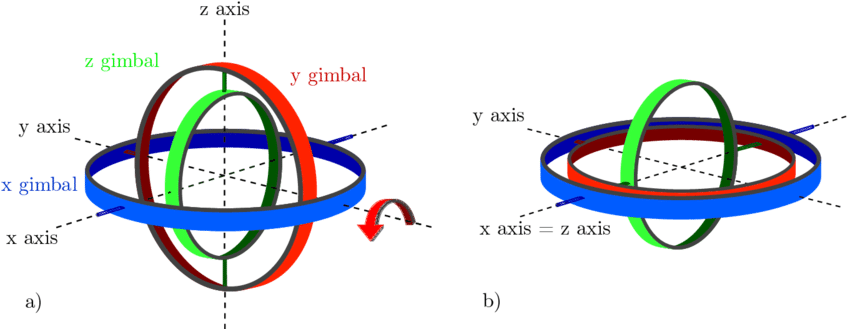
\includegraphics[width=0.8\textwidth]{../img/memoria/gimbal_lock.png}
	\caption[Ejemplo de \textit{gimbal lock}]{Ejemplo de \textit{gimbal lock}. Imagen extraída de ~\cite{gimbalimage}.}
	\label{img:gimballock}
\end{figure}

\section{Sistemas de colisiones y físicas en 3D}

En los entornos tridimensionales interactivos como los desarrollados en \textit{Unreal Engine}, la detección de colisiones y la simulación física juegan un papel fundamental tanto para la interacción con objetos como para la inmersión del usuario~\cite{unrealphysicsdocs}.

\subsubsection{Detección de colisiones}

La detección de colisiones es el proceso mediante el cual se determina si dos o más objetos en el espacio tridimensional se intersecan o entran en contacto. Para optimizar este cálculo, los motores como \textit{Unreal Engine} utilizan primitivas de colisión simplificadas (por ejemplo, cajas, esferas o cápsulas) en lugar de las mallas complejas de los modelos. Cada objeto puede tener uno o varios componentes de colisión que definen su comportamiento físico y de colisión en el mundo virtual.

Existen distintos canales de colisión y respuestas configurables:
\begin{itemize}
    \item \textbf{Bloqueo}: impide el paso del objeto.
    \item \textbf{Superposición}: detecta el contacto sin detener el movimiento.
    \item \textbf{Ignorar}: desactiva la colisión frente a determinados tipos de objetos.
\end{itemize}

Estas respuestas se configuran en el motor mediante el sistema de \textit{Collision Presets} y \textit{Object Channels}, permitiendo un control detallado sobre las interacciones entre objetos.

\subsubsection{Simulación física}

La simulación física busca replicar de manera realista el comportamiento de los objetos bajo leyes físicas básicas como la gravedad, la inercia, la fricción o los rebotes. \textit{Unreal Engine} emplea el motor físico \textit{Chaos Physics} para realizar estos cálculos en tiempo real.

Cada objeto puede tener activada o no la simulación física. Si está activada, se comporta como un cuerpo dinámico, reaccionando a fuerzas, colisiones y otras interacciones.

\section{Comunicación entre objetos en entornos visuales}

En el desarrollo de sistemas interactivos complejos dentro de \textit{Unreal Engine}, especialmente mediante \textit{Blueprints}, uno de los aspectos fundamentales es la capacidad de los distintos objetos (actores, componentes, interfaces) para comunicarse entre sí de manera eficiente, estructurada y mantenible. Esta comunicación define el flujo lógico del juego, la interacción del usuario con los elementos del entorno y la coordinación entre diferentes subsistemas del motor.

\subsection{Lógica basada en eventos}

El sistema de \textit{Blueprints} se apoya en un modelo orientado a eventos (\textit{event-driven}), en el cual los objetos reaccionan a estímulos como colisiones, entradas del usuario, temporizadores o condiciones personalizadas. Estos eventos se conectan con nodos de ejecución dentro del \textit{Graph Editor}, lo que permite definir respuestas visuales sin necesidad de programación textual en \textit{C++}~\cite{epicblueprintdocs}.

Entre los eventos más comunes se encuentran:
\begin{itemize}
  \item \texttt{BeginPlay}: se ejecuta al inicio del juego o cuando el actor es activado.
  \item \texttt{Tick}: se ejecuta cada fotograma y suele usarse para operaciones continuas.
  \item \texttt{OnOverlapBegin} / \texttt{OnHit}: se disparan en colisiones físicas o superposiciones.
  \item Eventos personalizados definidos por el usuario (\textit{Custom Events}).
\end{itemize}

\subsection{Interfaces en Blueprint}

Para garantizar un bajo acoplamiento entre elementos y fomentar la reutilización del código, \textit{Unreal Engine} proporciona el sistema de \textit{Blueprint Interfaces}. Estas permiten definir contratos de funciones sin necesidad de conocer la implementación exacta del otro objeto~\cite{millerblueprintcpp}.

Las interfaces son especialmente útiles cuando múltiples actores diferentes deben reaccionar a una misma instrucción sin necesidad de herencia múltiple. Por ejemplo, una interfaz \texttt{Interactuable} podría declarar una función \texttt{Interactuar()}, que luego implementen tanto puertas, botones como personajes no jugables.

\subsection{Despachadores de eventos (\textit{Event Dispatchers})}

Otra herramienta poderosa para la comunicación asíncrona entre objetos es el uso de \textit{Event Dispatchers}. Estos permiten declarar emisores de eventos personalizados dentro de un \textit{Blueprint}, que otros actores pueden suscribirse para ejecutar funciones concretas cuando se produzca el evento.

Este patrón de diseño tipo \textit{observador} facilita la coordinación entre componentes sin acoplamiento directo.

\subsection{Flujos condicionales y comunicación entre componentes}

Además de los mecanismos anteriores, el sistema de \textit{Blueprints} permite acceder directamente a componentes de otros actores mediante referencias explícitas. Aunque esta técnica es más directa, puede generar dependencias rígidas si no se usa con cautela.

Para casos sencillos o controlados, acceder a propiedades públicas de otro actor (por ejemplo, cambiar el color de una luz, activar una animación o reproducir un sonido) es una forma válida y eficaz de comunicación.

\subsection{Buenas prácticas de arquitectura}

Para evitar problemas de escalabilidad y errores difíciles de depurar, se recomienda:

\begin{itemize}
  \item Usar \textit{Interfaces} para definir comunicación entre clases distintas.
  \item Utilizar \textit{Dispatchers} cuando el evento debe propagar información a varios objetos.
  \item Minimizar referencias directas entre objetos no relacionados jerárquicamente.
  \item Modularizar la lógica en funciones reutilizables y macros claramente documentadas.
\end{itemize}

Estas herramientas permiten mantener un sistema organizado, extensible y coherente, especialmente en entornos de desarrollo visual como el que ofrece \textit{Unreal Engine}, donde el control sobre la ejecución y la interacción entre objetos es esencial para la calidad final del proyecto.
